
\documentclass{exam}

\usepackage{fullpage}
\usepackage{enumerate}
\usepackage{siunitx} 
\usepackage{graphicx}
\usepackage[fleqn]{amsmath}
\usepackage{cancel}
\usepackage{polynom}
\usepackage{float}
\usepackage{mdwlist}
\usepackage{booktabs}
\usepackage{cancel}
\usepackage{polynom}
\usepackage{caption}

\newcommand{\degree}{\ensuremath{^\circ}} 
\everymath{\displaystyle}

% \begin{figure}[H]
%   \centering
%   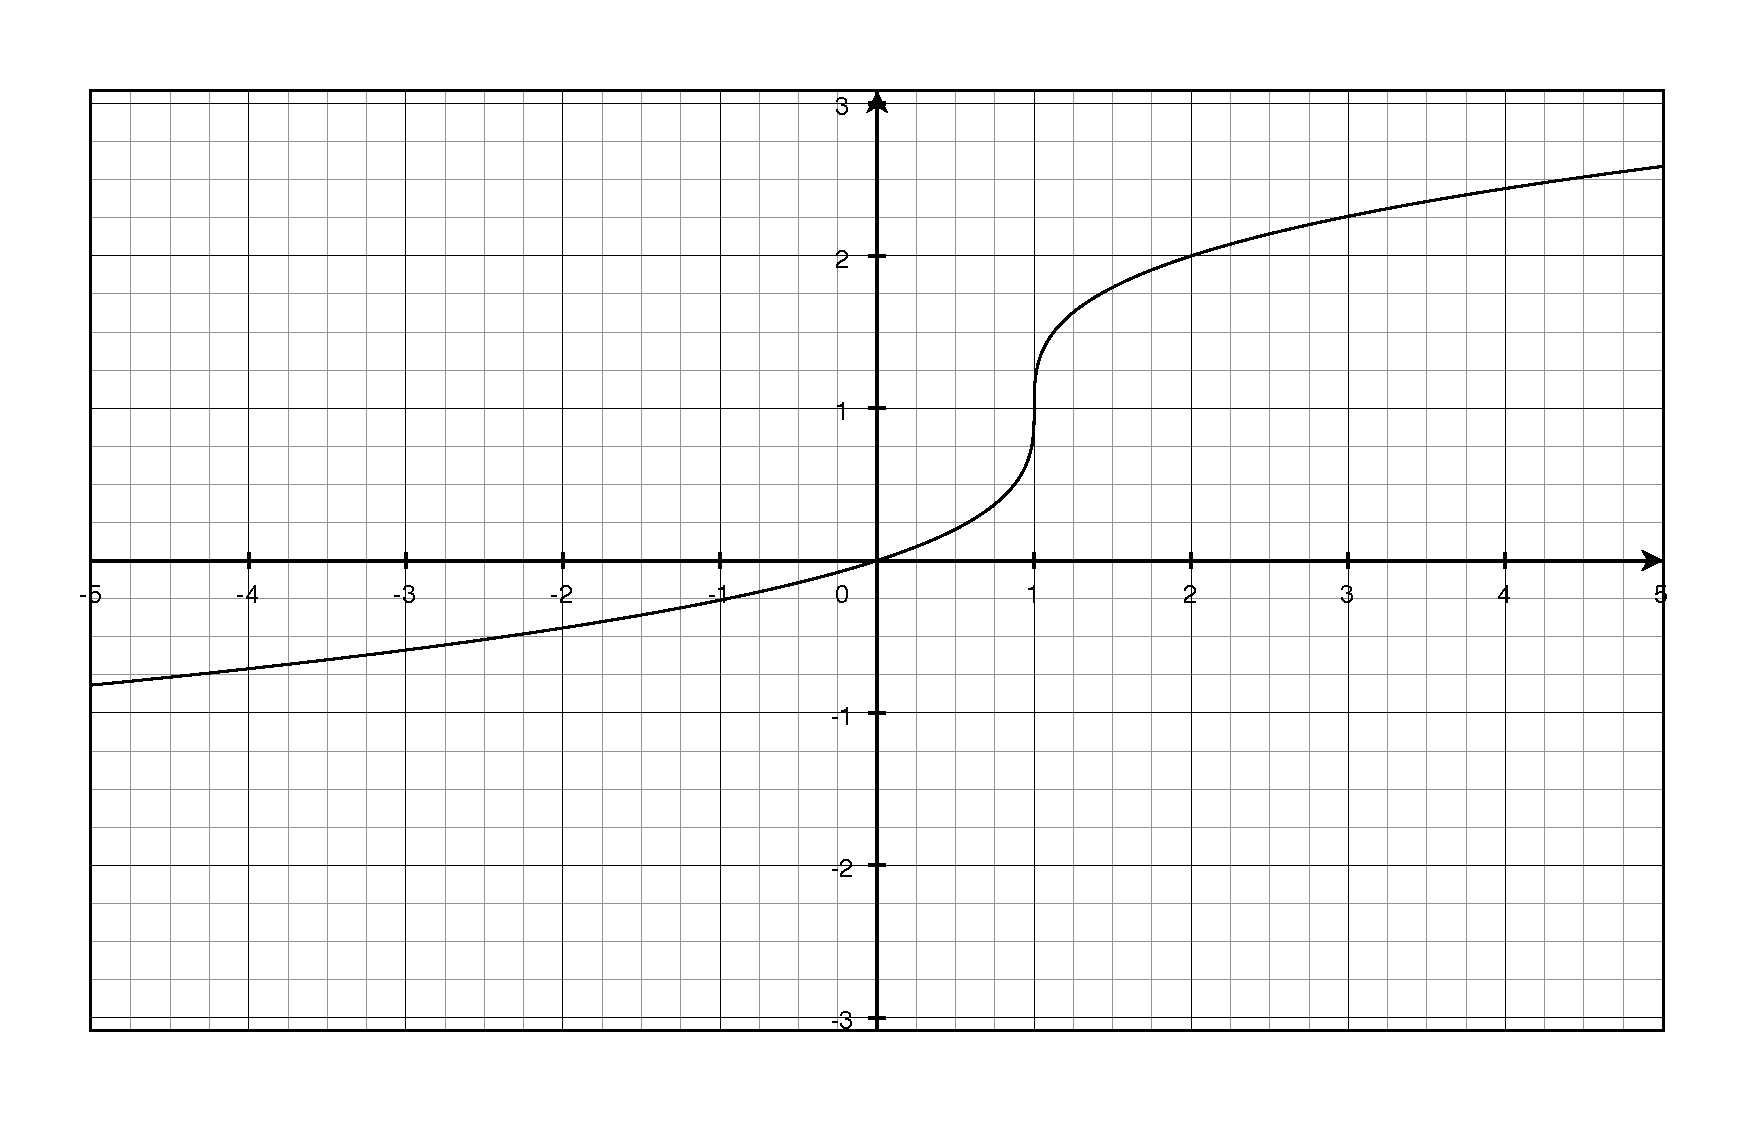
\includegraphics[scale=.3]{question7.eps}
%   \caption*{Question 7}
% \end{figure}

% \begin{tabular}{cc}
% \toprule
% period & amplitude \\
% \midrule
%   $\pi$ & $2$ \\
% \bottomrule
% \end{tabular}

% \textwidth 6.5 in

\printanswers

\ifprintanswers 
\usepackage{2in1, lscape} 
\fi

\title{Math 263a \\ Homework Two}
\date{January 25, 2012}

\begin{document}

\maketitle

\section{Homework}

\begin{itemize*}
  \item Read Section 2.2-2.3
  \item pp 54-55: 1-2, 4-5, 11, 15-16, 23, 28
  \item pp 61-65: 10-11, 14
\end{itemize*}

133 points possible

\section{Extra Credit}

pp 54-55: 24 (10 points) and 29 (5 points)

\ifprintanswers
\begin{description}
\item[24] (10 points)

\begin{enumerate}[(a)]
\item
To give the new function a name, let $g(x) = F(x) - F(-x)$.
\begin{align*}
  g(-x) &= F(-x) - F(x) \\
        &= - F(x) + F(-x)  \\
        &= -(F(x) - F(-x)) \\
        &= -g(x) \\
\end{align*}

\item
Let $h(x) = F(x) + F(-x)$.
\begin{align*}
  h(-x) &= F(-x) + F(x) \\
        &= F(x) + F(-x) \\
        &= h(x) \\
\end{align*}

\item $g(x)$ from part (a) is an odd function and $h(x)$ from (b) is an even function.  If we add them together, and do
  a little arithmetic, we can get $F$: 
\begin{align*}
  (g + h)(x) &= F(x) - F(-x) + F(x) + F(-x) \\
             &= 2 \cdot F(x) \\
  F(x)       &= \frac{1}{2} (g + h)(x)
\end{align*}
\end{enumerate}

\item[29] (5 points)
For the first hour, only plane A is moving.  For this hour, the distance is just A's rate or:
\[
  D(t) = 400t
\]

After the first hour, the planes form a right triangle.  Since the northbound plane has been flying the whole time, the
north leg of the triangle is: 
\[
  N(t) = 400t
\]

The eastbound plane is just getting started, so it's been travelling for one hour less, and it isn't travelling as quickly:
\[
  E(t) = 300(t - 1)
\]

The distance is the hypotenuse:
\begin{align*}
  d(t) &= \sqrt{N^2(t) + E^2(t)} \\
       &= \sqrt{400t)^2 + (300t - 300)^2} \\
       &= \sqrt{160,000t^2 + 90,000t^2 - 180,000t + 90,000} \\
       &= \sqrt{250,000 t^2  - 180,000t + 90,000} \\
\end{align*}

\end{description}

\section{Questions}

\subsection{Section 2.2}
\begin{description}
\item[1] (12 points)
\begin{enumerate}[(a)]

\item 
\begin{align*}
  (f + g)(x) &= x^2 + x + 3 \\
  (f + g)(2) &= 9 \\
\end{align*} 

\item 
\begin{align*}
  (f \cdot g)(x) &= x^2(x + 3) \\
  (f \cdot g)(0) &= 0 \\
\end{align*} 

\item 
\begin{align*}
  (g / f )(x) &= \frac{x^2}{x + 3} \\
  (g / f )(3) &= \frac{3}{2} \\
\end{align*} 

\item 
\begin{align*}
  (f \circ g)(x) &= x^2 + 3 \\
  (f \circ g)(1) &= 4 \\
\end{align*} 

\item 
\begin{align*}
  (g \circ f)(x) &= (x + 3)^2 \\
  (g \circ f)(1) &= 16 \\
\end{align*} 

\item 
\begin{align*}
  (g \circ f)(x) &= (x + 3)^2 \\
  (g \circ f)(-8) &= 25 \\
\end{align*} 

\end{enumerate}

\item[2] (12 points)
\begin{enumerate}[(a)]

\item 
\begin{align*}
  (f - g)(x) &= x^2 + x - \frac{2}{x+3} \\
  (f - g)(2) &= 4 + 2 - \frac{2}{5} \\
             &= \frac{28}{5} \\
\end{align*} 

\item 
\begin{align*}
  (f/g)(x) &= \frac{(x^2 + x)(x+3)}{2} \\
  (f/g)(1) &= \frac{(2)(4)}{2} \\
           &= 4 \\
\end{align*} 

\item 
\begin{align*}
  (g^2)(x) &= \left( \frac{2}{(x+3)} \right)^2 \\
  (g^2)(3) &= \left( \frac{2}{6} \right)^2\\
           &= \frac{1}{9} \\
\end{align*} 

\item 
\begin{align*}
  (f \circ g)(x) &= \left( \frac{2}{x+3} \right)^2 + \frac{2}{x+3} \\
  (f \circ g)(1) &= \left( \frac{2}{4} \right)^2 + \frac{2}{4} \\
                 &= \frac{3}{4} \\
\end{align*} 

\item 
\begin{align*}
  (g \circ f)(x) &= \frac{2}{x^2 + x + 3} \\
  (g \circ f)(1) &= \frac{2}{5} \\
\end{align*} 

\item 
\begin{align*}
  (g \circ g)(x) &= \frac{2}{\left( \cfrac{2}{x+3} + 3 \right)} \\
                 &= \frac{2}{\left( \cfrac{3x + 11}{x+3} \right)} \\
                 &= \frac{2x + 6}{3x + 11} \\
                 \\
  (g \circ g)(3) &= \frac{6 + 6}{9 + 11} \\
                 &= \frac{3}{5} \\
\end{align*} 

\end{enumerate}

\item[4] (20 points)
\begin{enumerate}[(a)]

\item 
\[
  (f \cdot g)(x) = \frac{2\sqrt{x^2-1}}{x}
\]
The numerator must satisfy:
\begin{align*} 
  x^2-1 &\geq 0 \\
  x^2   &\geq 1 \\
\end{align*} 

So the domain is: $x \leq -1$ or $x \geq 1$.

\item
\[
  f^4(x) + g^4(x) = (x^2-1)^2 + \frac{16}{x^4}
\]

domain: $x \neq 0$

\item
\[
  (f \circ g)(x) = \sqrt{\frac{4}{x^2} - 1}
\]

domain:
\begin{align*}
  \frac{4}{x^2} - 1 &\geq 0 \\
  \frac{4}{x^2}     &\geq 1 \\
  x^2               &\leq 4 \\
\end{align*}

domain: $-2 \leq x \leq 2$ and $x \neq 0$

\item
\[
  (g \circ f)(x) = \frac{2}{\sqrt{x^2-1}}
\]

domain:
\begin{align*}
  x^2 - 1 &> 0 \\
  x^2 &> 1 \\
\end{align*}

domain: $x < -1$ or $x > 1$

\end{enumerate}

\item[5] (20 points)
\begin{enumerate}[(a)]

\item
\begin{align*}
  (f \circ g)(x) &= \sqrt{(| 1 + x |)^2 - 4} \\
                 &= \sqrt{x^2 + 2x - 3} \\
\end{align*}

\item
\begin{align*}
  (g \circ f)(x) &= \left| 1+\sqrt{x^2 - 4} \right| \\
                 &= 1+\sqrt{x^2 - 4} \\
\end{align*}

\end{enumerate}

\item[11] (10 points)
\begin{enumerate}[(a)]

\item
\begin{align*}
  f(x) &= x + 7 \\
  g(x) &= \sqrt{x} \\
\end{align*}

\item
\begin{align*}
  f(x) &= x^2 + x \\
  g(x) &= x^{15} \\
\end{align*}

\end{enumerate}

\pagebreak

\item[15] (5 points)

This is the graph of $f(x) = x^2$ shifted down 3 and right 2.

\begin{figure}[H]
  \centering
  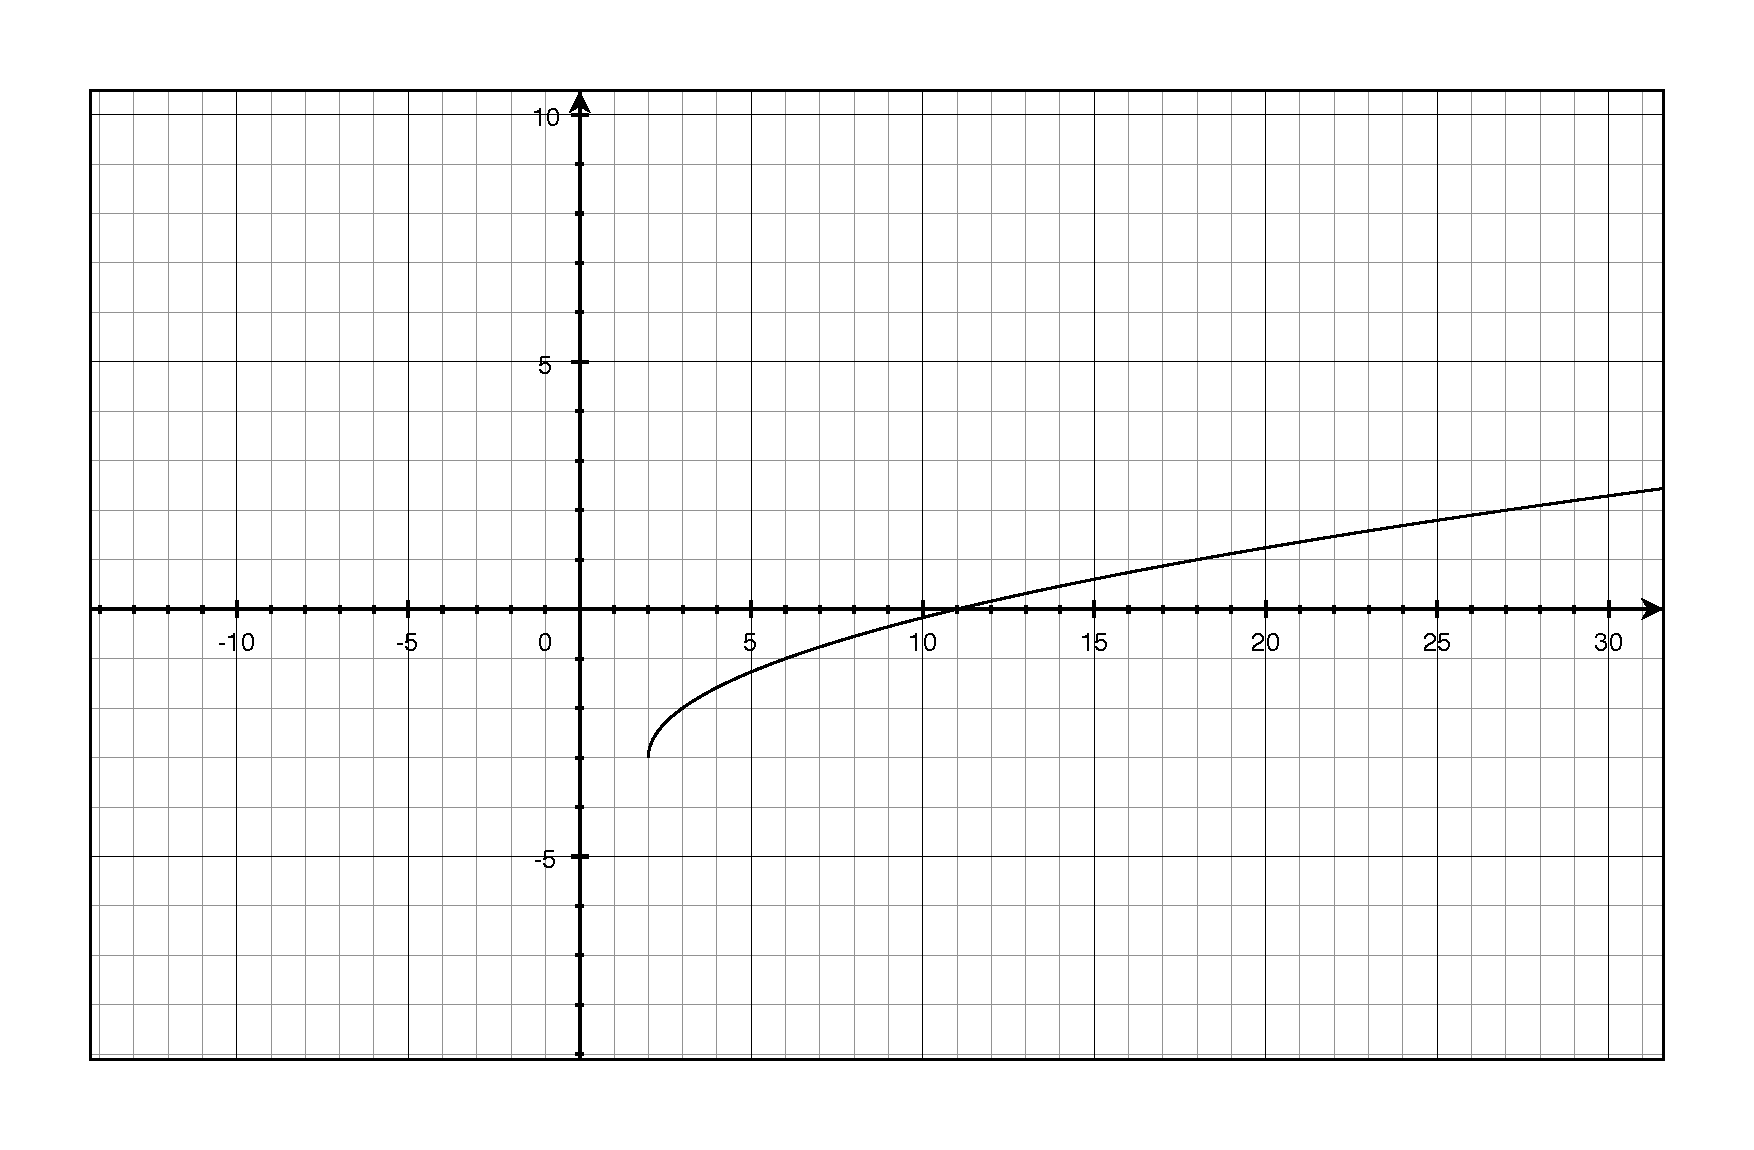
\includegraphics[scale=.3]{question_15.eps}
  \caption*{Question 15}
\end{figure}

\item[16] (5 points)
This is the graph of $f(x) = |x|$ shifted down 4 and left 3.

\begin{figure}[H]
  \centering
  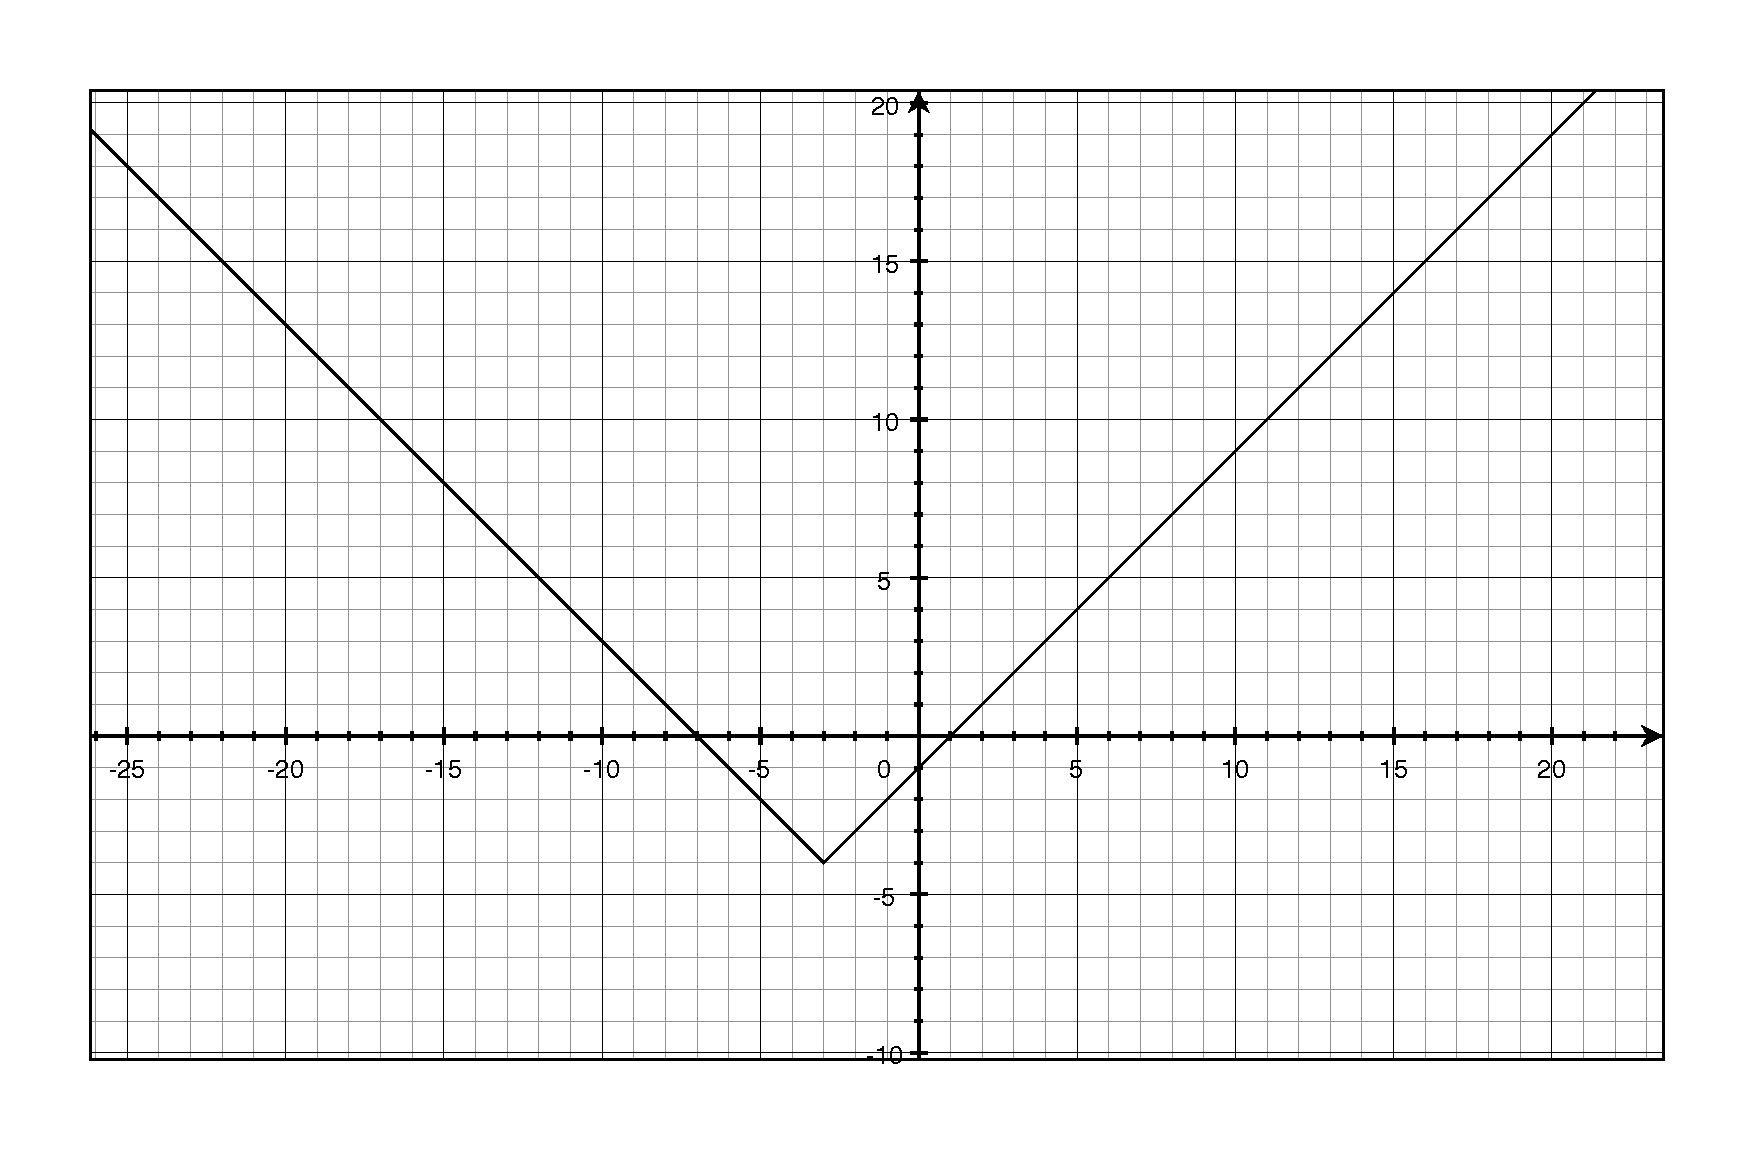
\includegraphics[scale=.3]{question_16.eps}
  \caption*{Question 16}
\end{figure}

\pagebreak

\item[23] (10 points)
I'll call the e function $e(x)$ and the odd function $o(x)$.

From the definitions of even and odd functions:
\begin{align*}
  e(-x) &= e(x) \\
  o(-x) &= -o(x) \\
\end{align*}

\begin{enumerate}[(a)]

\item
\begin{align*}
  f(x) &= e(x) + e(x) \\
  f(-x) &= e(-x) + e(-x) = e(x) + e(x) = f(x)
\end{align*}
$f$ is even

\item
\begin{align*}
  f(x) &= o(x) + o(x) \\
  f(-x) &= o(-x) + o(-x) = -o(x) - o(x) = -f(x)
\end{align*}
$f$ is odd

\item
\begin{align*}
  f(x) &= e(x) \cdot e(x) \\
  f(-x) &= e(-x) \cdot e(-x) = e(x) \cdot e(x) = f(x)
\end{align*}
$f$ is even

\item
\begin{align*}
  f(x) &= o(x) \cdot o(x) \\
  f(-x) &= o(-x) \cdot o(-x) = (- o(x)) \cdot (- o(x)) = f(x)
\end{align*}
$f$ is even

\item
\begin{align*}
  f(x) &= e(x) \cdot o(x) \\
  f(-x) &= e(-x) \cdot o(-x) = e(x) \cdot (- o(x)) = -f(x)
\end{align*}
$f$ is odd

\end{enumerate}

\item[28]
The two functions are for units and price:
\begin{align*}
  u(t) &= 120 + 2t + 3t^2 \\
  p(t) &= 6000 + 700t \\
\end{align*}

The revenue depends on how many units he makes and the price for each unit:
\begin{align*}
  r(t) &= (u \cdot p)(t) \\
       &= (120 + 2t + 3t^2)(6000 + 700t) \\
\end{align*}

\end{description}

\pagebreak

\subsection{Section 2.3}
\begin{description}
\item[10] (12 points)
\begin{enumerate}[(a)]
\item $\tan \left( \frac{\pi}{3} \right) = \frac{ \sin \left( \cfrac{\pi}{3} \right)} {\cos \left( \cfrac{\pi}{3} \right)}  = \sqrt{3}$
\item $\sec \left( \frac{\pi}{3} \right) = \frac{1} {\cos \left( \cfrac{\pi}{3} \right)}  = 2$
\item $\cot \left( \frac{\pi}{3} \right) = \frac{1}{\tan \left(\cfrac{\pi}{3}\right)} = \frac{\sqrt{3}}{3}$
\item $\csc \left( \frac{\pi}{4} \right) = \frac{1}{\sin \left(\cfrac{\pi}{4}\right)} = \sqrt{2}$
\item $\tan \left( - \frac{\pi}{6} \right) = \frac{ \sin \left( -\cfrac{\pi}{6} \right)} {\cos \left( -\cfrac{\pi}{6} \right)}  = -\frac{\sqrt{3}}{3}$
\item $\cos \left( -\frac{\pi}{3} \right) = \cos \left( \frac{\pi}{3} \right) = \frac{1}{2}$
\end{enumerate}

\item[11] (10 points)
\begin{enumerate}[(a)]
\item
\begin{align*}
  (1 + \sin z)  (1 - \sin z) &= 1 - \sin^2 z \\
  &= \cos^2 z \\
  &= \frac{1}{\sec^2 z} \\
\end{align*}

\item
\begin{align*}
  (\sec t - 1)  (\sec t + 1) &= \sec^2 t - 1 \\
  &= \tan^2 t \\
\end{align*}

\item
\begin{align*}
  \sec t - \sin t \tan t &= \frac{1}{\cos t} - \frac{\sin^2 t}{\cos t} \\
  &= \frac{1}{\cos t}(1 - \sin^2 t) \\
  &= \frac{1}{\cos t}(\cos^2 t) \\
  &= \cos t \\
\end{align*}

\item
\begin{align*}
  \frac{sec^2 t - 1}{\sec^2 t} &= \frac{\sec^2 t}{\sec^2 t} - \frac{1}{\sec^2 t} \\
    &= 1 - \frac{1}{\sec^2 t} \\
    &= 1 - \cos^2 \\
    &= \sin^2 t \\
\end{align*}

\item
\begin{align*}
  \cos t(\tan t + \cot t) &= \cos t \left( \frac{\sin t}{\cos t} + \frac{\cos t}{\sin t} \right) \\
  &= \sin t + \frac{\cos^2 t}{\sin t} \\
  &= \frac{\sin^2 t + \cos^2 t}{\sin t} \\
  &= \frac{1}{\sin t} \\
  &= \csc t \\
\end{align*}

\end{enumerate}

\item
\begin{figure}[H]
  \centering
  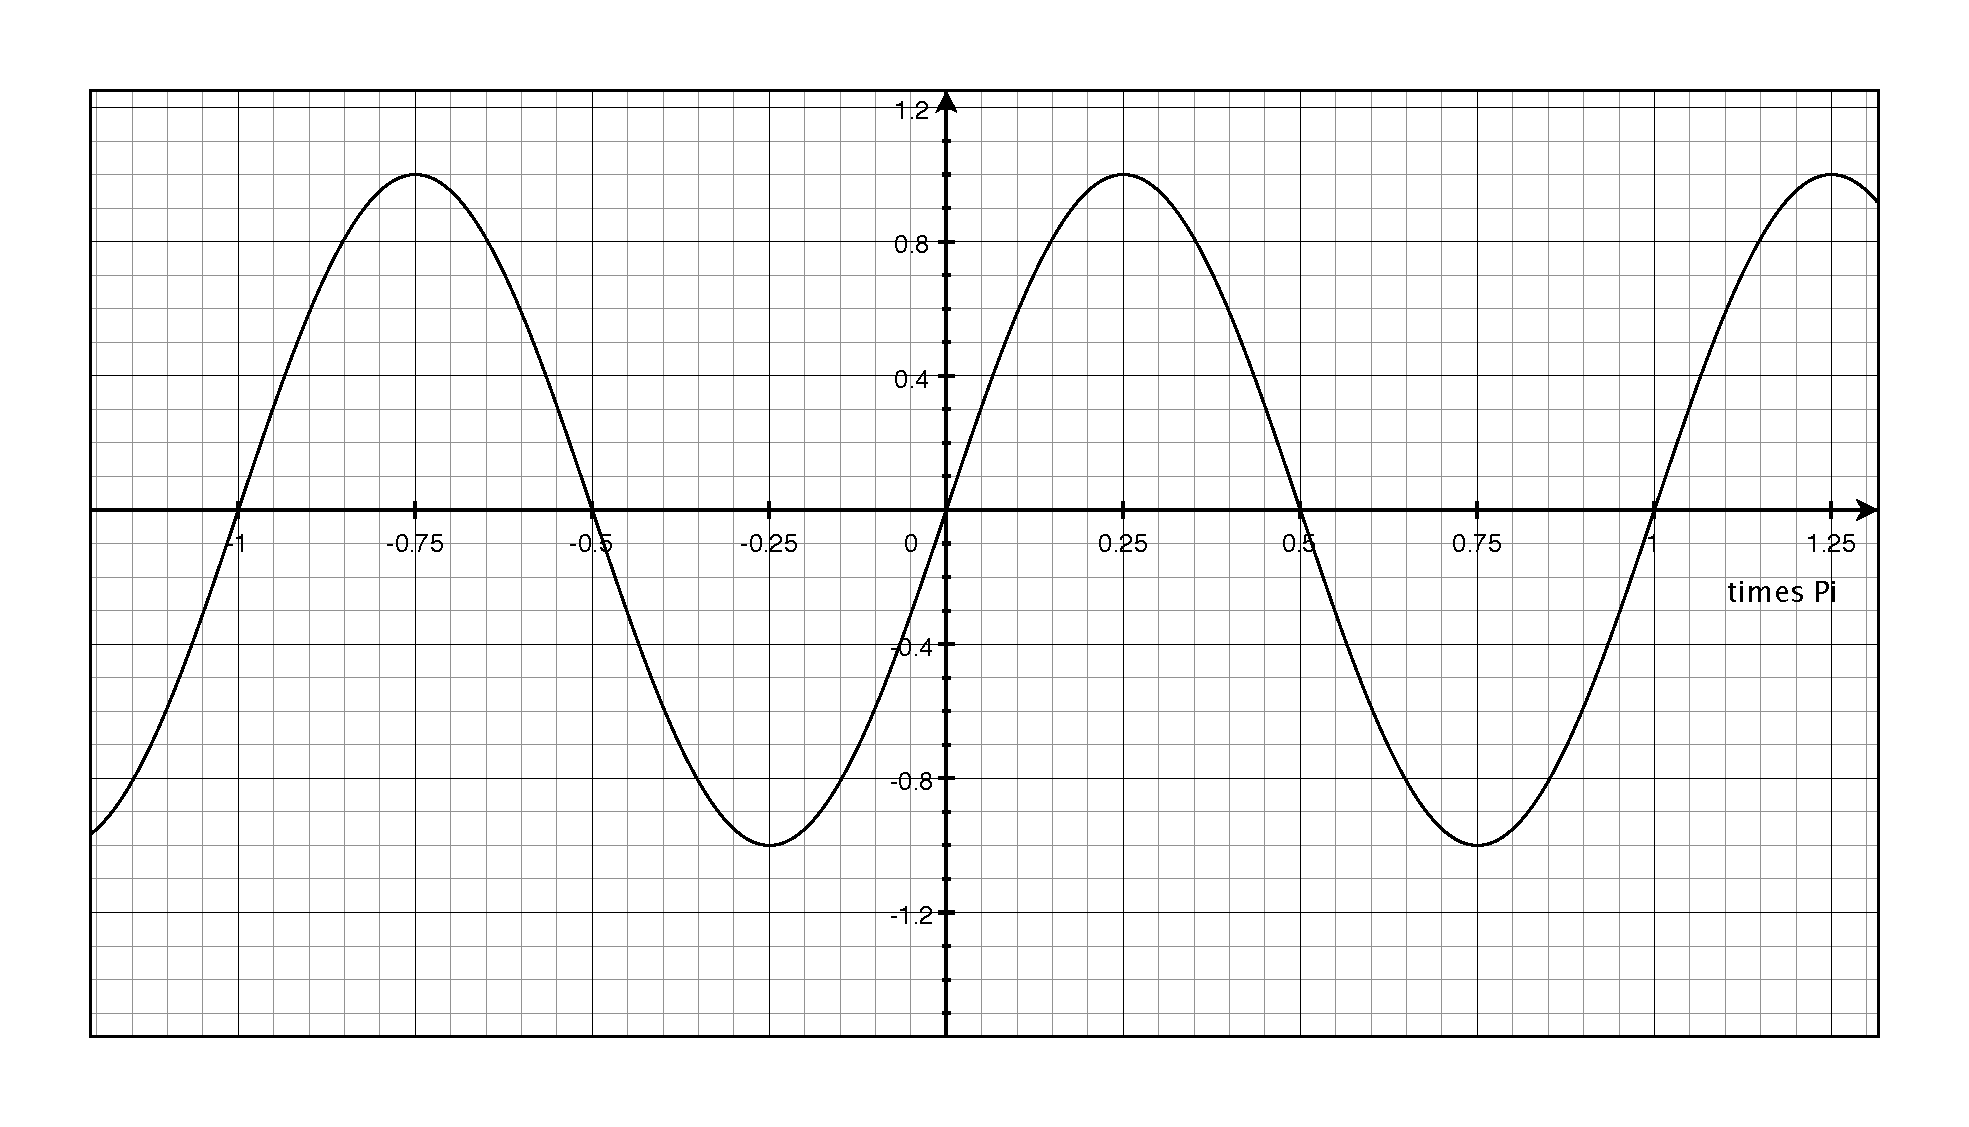
\includegraphics[scale=.3]{question_14a.eps}
  \caption*{Question 14a (5 points)}
\end{figure}

\item
\begin{figure}[H]
  \centering
  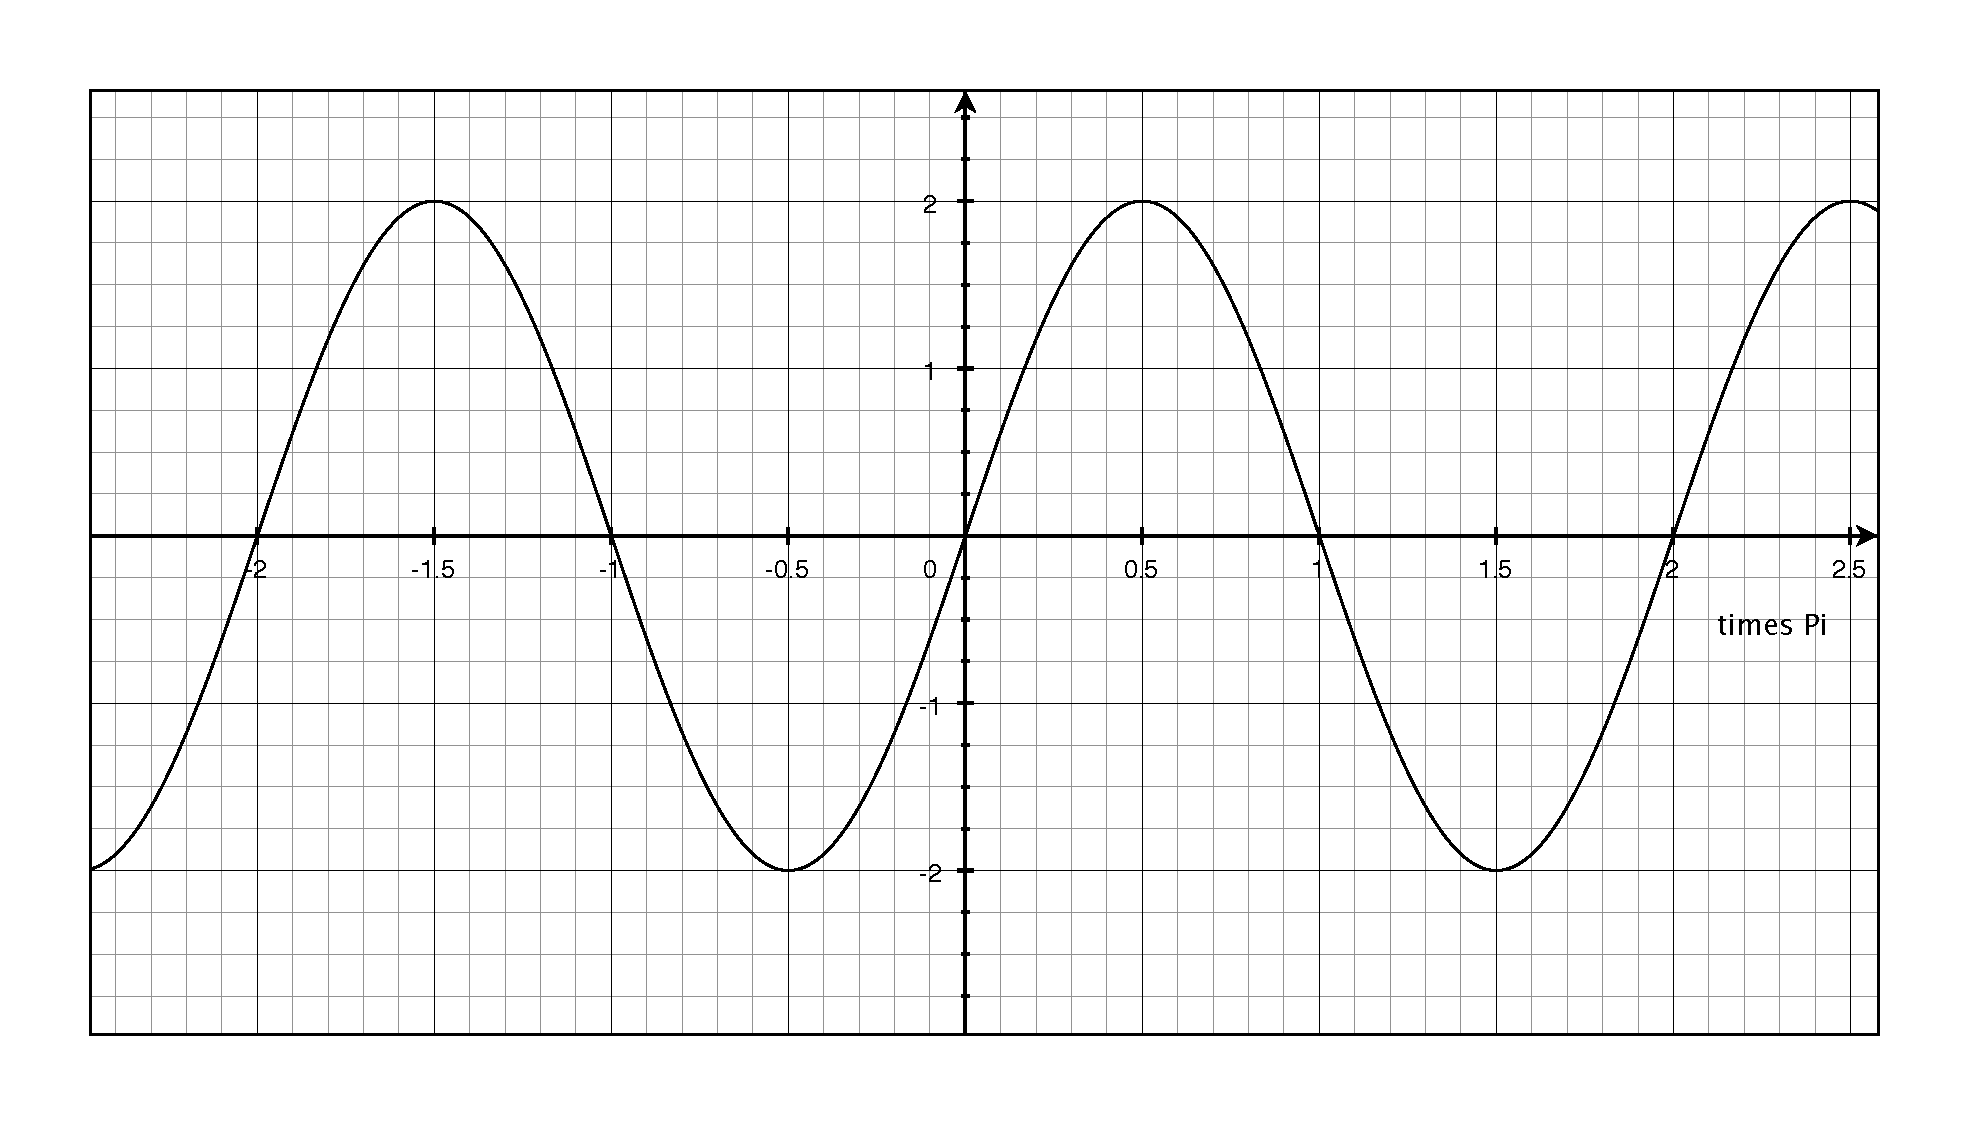
\includegraphics[scale=.3]{question_14b.eps}
  \caption*{Question 14b (5 points)}
\end{figure}

\item
\begin{figure}[H]
  \centering
  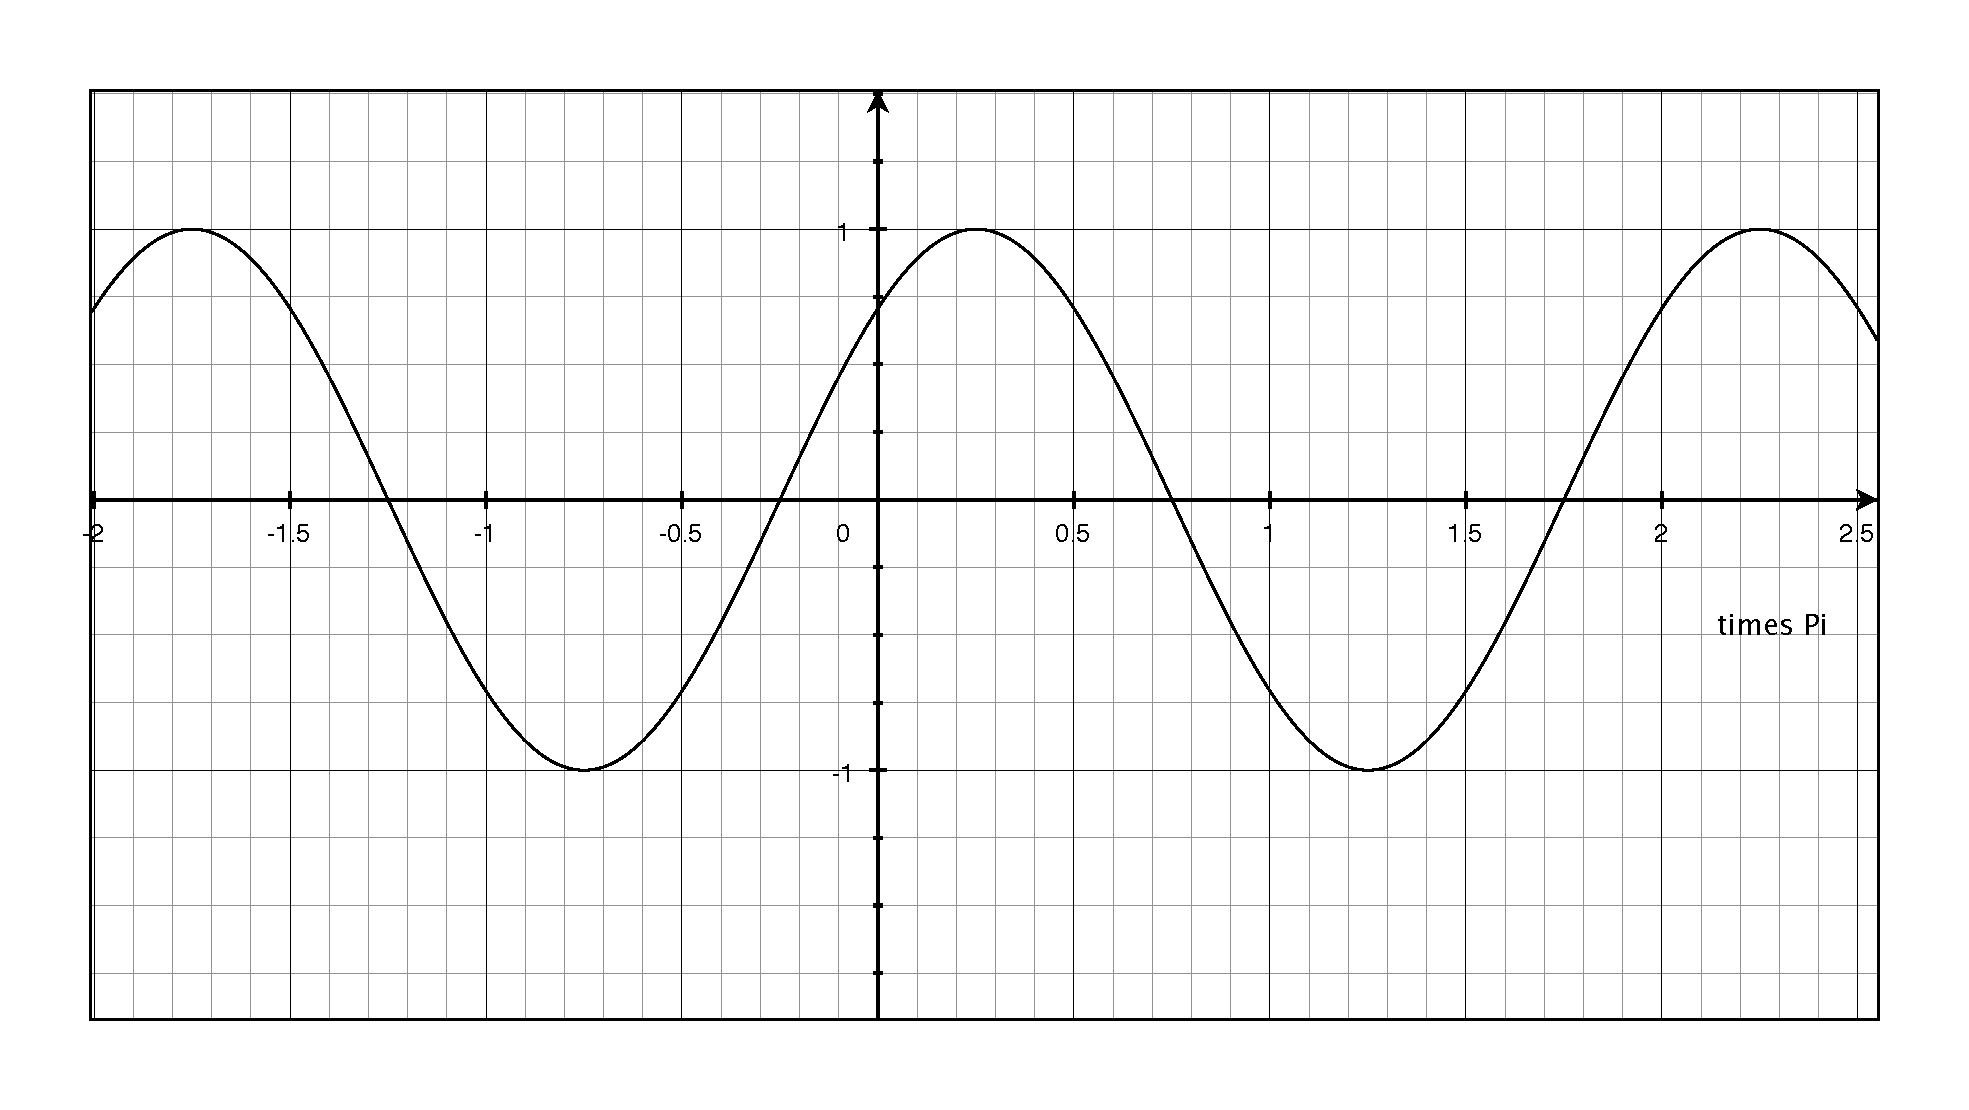
\includegraphics[scale=.3]{question_14c.eps}
  \caption*{Question 14c (5 points)}
\end{figure}

\item
\begin{figure}[H]
  \centering
  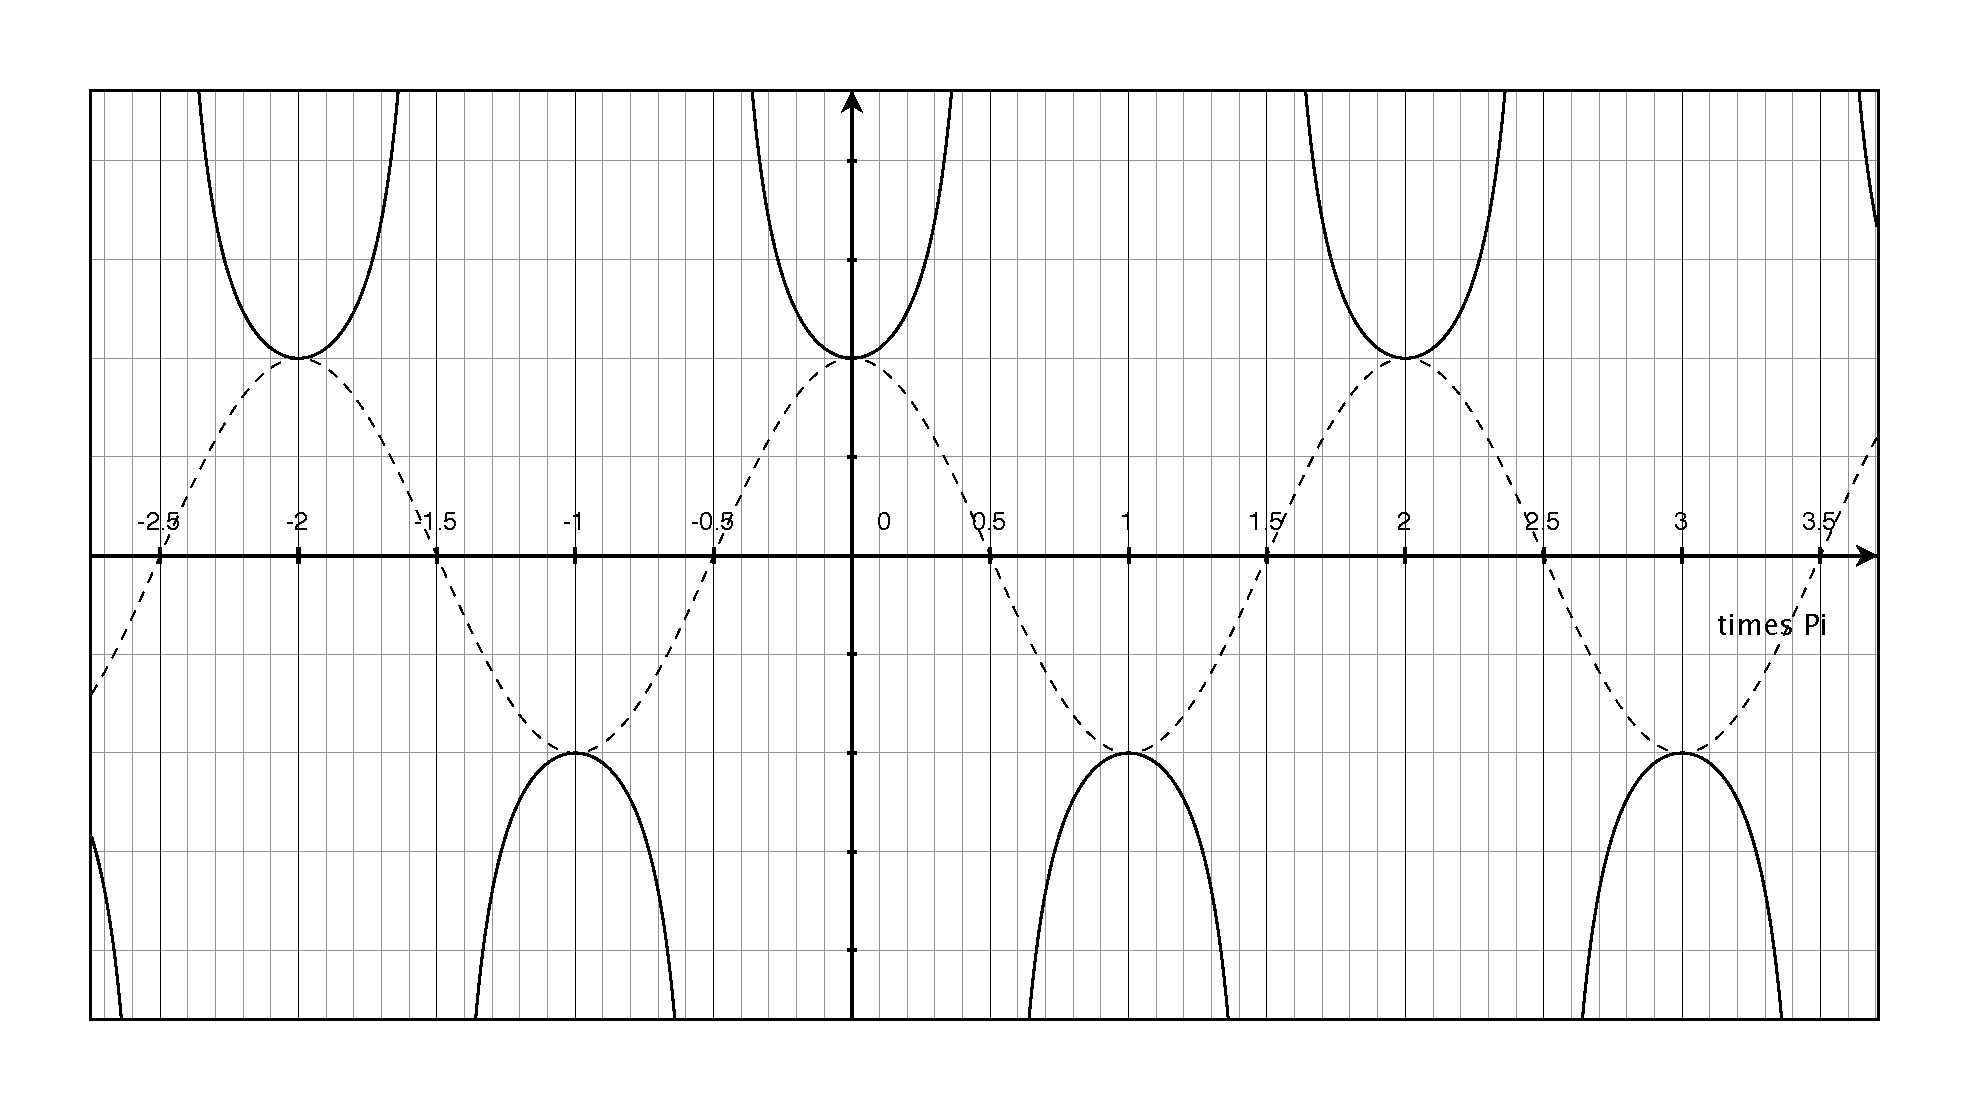
\includegraphics[scale=.3]{question_14d.eps}
  \caption*{Question 14d (5 points)}
\end{figure}



\end{description}

\else

\vspace{8 cm}

{\em When I speak, I don't speak as a Democrat, or a Republican...I speak as a victim of America's so-called democracy. You
  and I have never seen democracy; all we've seen is hypocrisy. When we open our eyes today and look around America, we
  see America not through the eyes of someone who has enjoyed the fruits of Americanism, we see America
  through the eyes of someone who has been the victim of Americanism. We don’t see any American dream; we've experienced
  only the American nightmare. We haven't benefited from America's democracy; we've only suffered from America's
  hypocrisy. And the generation that's coming up now can see it and are not afraid to say it.}

\vspace{.2 cm}

\hspace{1 cm} --Malcolm X

\fi

\end{document}

